\section{Durchführung}
\label{sec:Durchführung}

Für den Versuchsaufbau wird ein elektrisches Thermometer, eine Heizplatte, zwei Messbecher und ein Thermobehälter, sowie die verschiedenen Materialien benötigt.
In \autoref{fig:aufbau} ist der Aufbau dargestellt.

\begin{figure}[htbp]
    \centering
    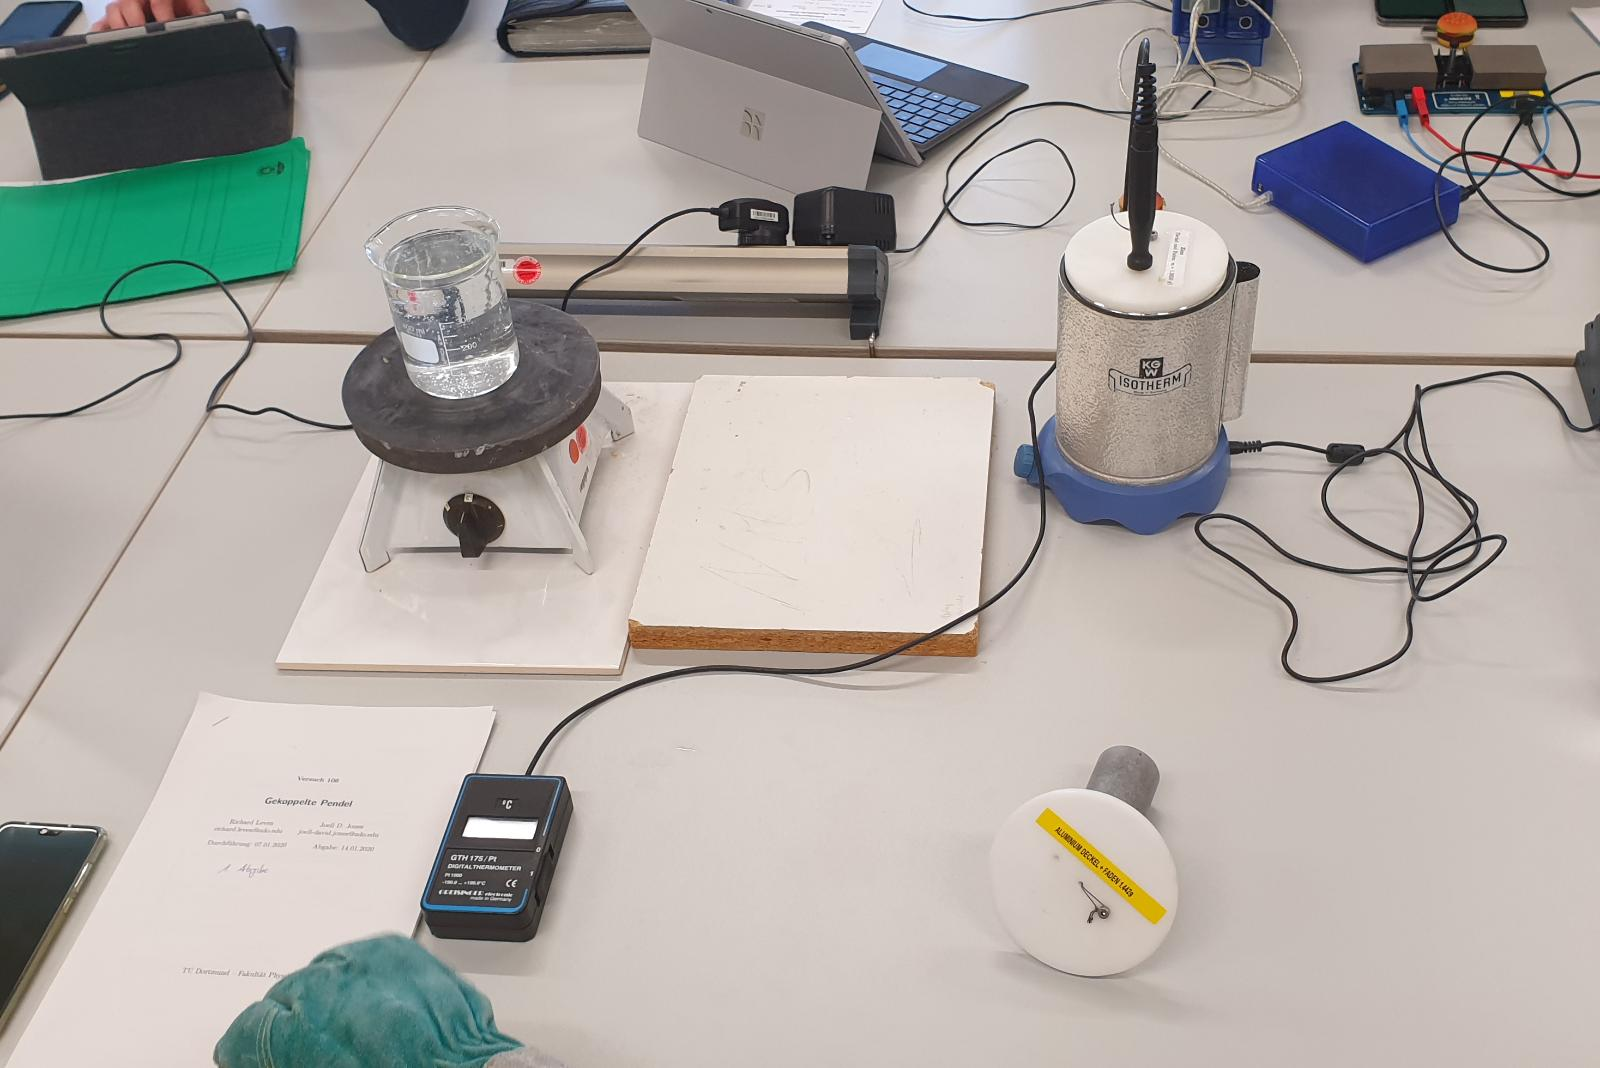
\includegraphics[width=\textwidth]{content/Bilder/Aufbau.jpg}
    \caption{Aufbau des Experiments.}
    \label{fig:aufbau}
\end{figure}


Es wird für alle drei Materialien eine gleiche Versuchsabfolge durchgeführt.\\
Zuerst wird mit einer Präzisionswaage die Masse aller drei Stoffe gemessen.
Danach werden die Materialien einzeln und der Reihe nach in einem Wasserbad auf $80°C$ erhitzt.
Die heiße Probe wird dann in ein Wasserbad mit einer Anfangstemperatur getaucht.
Sobald das Wasser die Wärme des Materials vollständig aufgenommen hat und nicht mehr ansteigt, wird der Wert notiert.
Es wird ebenfalls das Gewicht des Wassers im Thermobehälter, sowie die Wärmekapazität des Thermobehälters selbst gemessen.
Für Aluminium und Zinn werden diese Messungen je drei mal durchgeführt, für Graphit nur einmal.\\
\newpage

\autoref{fig:tab} zeigt die verschiedenen vorgegebenen Größen der Materialien.
\begin{figure}[htbp]
    \centering
    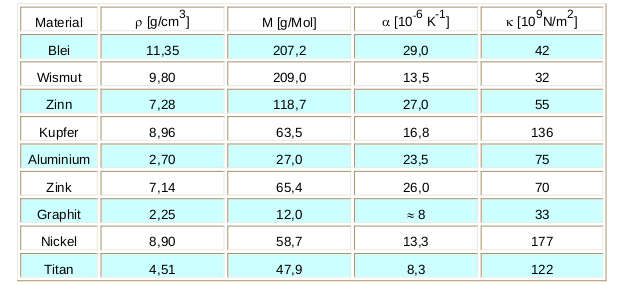
\includegraphics[width=\textwidth]{content/Bilder/Tabelle.png}
    \caption{Materialdaten für mehrere Stoffe.}
    \label{fig:tab}
\end{figure}